\documentclass[conference]{IEEEtran}

% ---- パッケージ ----
\usepackage{graphicx}
\usepackage{amsmath}
\usepackage{siunitx}

% フォント(XeLaTeX + IEEEtran での ptm 警告対策)
\usepackage{newtxtext}
\usepackage{newtxmath}

% ハイパーリンクは最後
\usepackage[hidelinks]{hyperref}

% ---- タイトル・著者 ----
\title{Historical Case Study: 0.25-$\mu$m 64-Mbit DRAM Ramp-up and Pseudo-SRAM (VSRAM)}

\author{
\IEEEauthorblockN{Shinichi Samizo}
\IEEEauthorblockA{Independent Semiconductor Researcher\\
Project Design Hub, Samizo-AITL\\
\textit{Email:} \href{mailto:shin3t72@gmail.com}{shin3t72@gmail.com}\quad
\textit{GitHub:} \href{https://github.com/Samizo-AITL}{Samizo-AITL}}
}

\begin{document}
\maketitle

% ---- Abstract ----
\begin{abstract}
This paper presents a flagship proof-of-concept humanoid robot control system that integrates
finite state machines (FSM), proportional-integral-derivative (PID) controllers, state-space methods
(LQR/LQG), and large language models (LLMs) into a unified three-layer architecture. 
Unlike existing humanoid platforms such as Boston Dynamics Atlas and Tesla Optimus,
our approach emphasizes autonomy, fault tolerance, and sustainability.

The proposed architecture is realized as a cross-node chipset design: 
a 22 nm SoC executes LLM inference, FSM management, and state-space control;
a 0.18 µm AMS sensor hub processes multimodal inputs (vision, IMU, force, audio);
and a 0.35 µm LDMOS power drive with external GaN/MOSFET chips delivers high-torque actuation.
Energy harvesting via piezoelectric, photovoltaic, and regenerative methods 
extends operational lifetime in off-grid environments.

System-level modeling and verification are performed using SystemDK, 
demonstrating posture recovery within 200 ms, gait stability improved by 30\% over PID-only control,
and energy efficiency gains of 15\% with hybrid control and harvesting. 
Checkpointing with FRAM/EEPROM further enables fast resume ($\leq$10 ms) and robust mission continuity. 
These results highlight the feasibility of a sustainable and resilient humanoid control system
that bridges advanced control theory with emerging AI techniques.

\end{abstract}


% ---- Sections ----
\section{Introduction}

In the late 1990s, Japan's semiconductor industry was in transition. At Epson's Sakata 8-inch fab, DRAM was \emph{not} pursued as an end business; rather, DRAM technology transfer was used as a \textbf{strategic vehicle} to absorb submicron process technologies at and beyond 0.35~\si{\micro\meter} and redeploy them into Epson's core devices (ASICs, logic ICs, display drivers, and inkjet driver ICs).

The technology transfer from Mitsubishi covered three nodes, each with a clear role:
(1) 0.5~\si{\micro\meter} 16~Mbit DRAM --- to establish mass-production capability and stabilize fab operation; 
(2) 0.35~\si{\micro\meter} 64~Mbit DRAM (2nd gen) --- to introduce a scaled process while tackling yield window narrowing; 
(3) 0.25~\si{\micro\meter} 64~Mbit DRAM (3rd gen) --- as the next-stage validation bed and the basis for in-house deployment.

This paper focuses on the 0.25~\si{\micro\meter} (3rd gen) ramp-up in 1998: a process overview, the ramp-up method, and a failure-analysis–driven yield-improvement cycle. We also trace how these results enabled the 0.25~\si{\micro\meter} mobile pseudo-SRAM (VSRAM) in 2001 and why trench-based 0.18~\si{\micro\meter} VSRAM was abandoned.

We summarize cell/circuit features of the 0.25-\textmu m 64-Mbit DRAM (stack capacitor, divided word-line, WSi stacks), and the wafer-test binning (Bin1--Bin7). For VSRAM, SRAM-like access is achieved by internal refresh logic while keeping DRAM cells; mobile-grade operation extended the temperature guarantee from 80~\si{\celsius} to 90~\si{\celsius}.

\section{Process Overview and Ramp-up Method}

\subsection{Process Overview (0.25-\si{\micro\meter} 64~Mbit DRAM, 3rd Gen)}

\begin{itemize}
  \item \textbf{Lithography}: First adoption of a KrF stepper for 0.25-\si{\micro\meter} volume exposure.
  \item \textbf{Isolation}: Semi-recess LOCOS.
  \item \textbf{Wells}: Triple-well with Deep N-Well to improve cell noise immunity.
  \item \textbf{Word-Line Gate Electrode}: CVD tungsten silicide (WSi). A dielectric \textbf{barrier cap (BRAC)} sits atop the WL stack, providing etch robustness and insulation.
  \item \textbf{Bit Line}: \emph{Self-aligned contact} --- the bit-line contact and the bit line are formed simultaneously by WSi-CVD; the BRAC blocks contact-to-WL shorts.
  \item \textbf{Storage Node Capacitor}: Stacked capacitor; surface roughening yields $\sim$1.5–1.8$\times$ capacitance gain.
  \item \textbf{Metallization/Passivation}: AlCu/TiN interconnect; SOG planarization; SiN or PI passivation.
\end{itemize}

\subsection{Ramp-up Method}

The node transfer followed a factory-wide, fast-turn scheme:

\paragraph{Base flow: SCF $\rightarrow$ shape lots $\rightarrow$ production lots}
\begin{enumerate}
  \item \textbf{Short Cycle Feedback (SCF)}: Each unit process (diffusion, CVD/PVD, etch, etc.) runs short-cycle wafers per its ramp-up spec to quickly evaluate and lock conditions.
  \item \textbf{Shape lots ($\sim$10 lots)}: Provide \emph{real product wafers} to unit teams for items only assessable on full stacks and, in parallel, (i) verify photo CDs, (ii) photo$\to$etch CD transfer, and (iii) cross-sections after interlayer films. Recipes are updated for following lots.
  \item \textbf{Production (reliability) lots}: Multiple lots for wafer test and long-term reliability (incl.\ burn-in) to judge mass-production readiness.
\end{enumerate}

\paragraph{Practical flow (author's role)}
Process conditions (two floppy disks) were received from the mother fab and deployed to unit teams; each team executed SCF and fed back updates. The author consolidated the latest settings into the \emph{electronic traveler}, launched $\sim$10 shape lots, fixed target CDs/films, and then ran 5 reliability lots for E-test and reliability signoff.

\paragraph{Operations to compress schedule}
Normal lots use stocker $\leftrightarrow$ rail transfer and queue at tools. For critical first-pass lots, we used \textbf{hand-carry flow}: engineers delivered cassettes to tools with operators standing by, eliminating transfer/queue loss. Even so, a full pass took about two months; the entire ramp spanned $\sim$5 months. Daily morning meetings posted a laminated traveler on a whiteboard to visualize lot progress, schedule slip (in days), and unit-team status. Technical staff also operated in a two-shift scheme (day/night) to sustain 24/7 feedback.

\section{Results and Discussion}
System-level simulation was performed with representative AI inference workloads.

\subsection{Standby Power}
Migrating cold data and checkpoints to the FeRAM-backed tier yields more than 30\% reduction in standby power.
This reduction arises from suppressing periodic DRAM refresh for inactive regions.

\subsection{Resume Latency}
FeRAM allows direct restore of checkpoints without full DRAM wake-up.
Resume latency is reduced to the $\mu$s range, enabling near-instant resume after power gating and improving energy efficiency for mobile edge AI.

\subsection{Endurance}
FeRAM endurance of $10^{12}$~writes/year fits within FeRAM capability for checkpoint traffic.

% ===== Fig.2: Access time vs. Retention =====
\begin{figure}[!t]
\centering
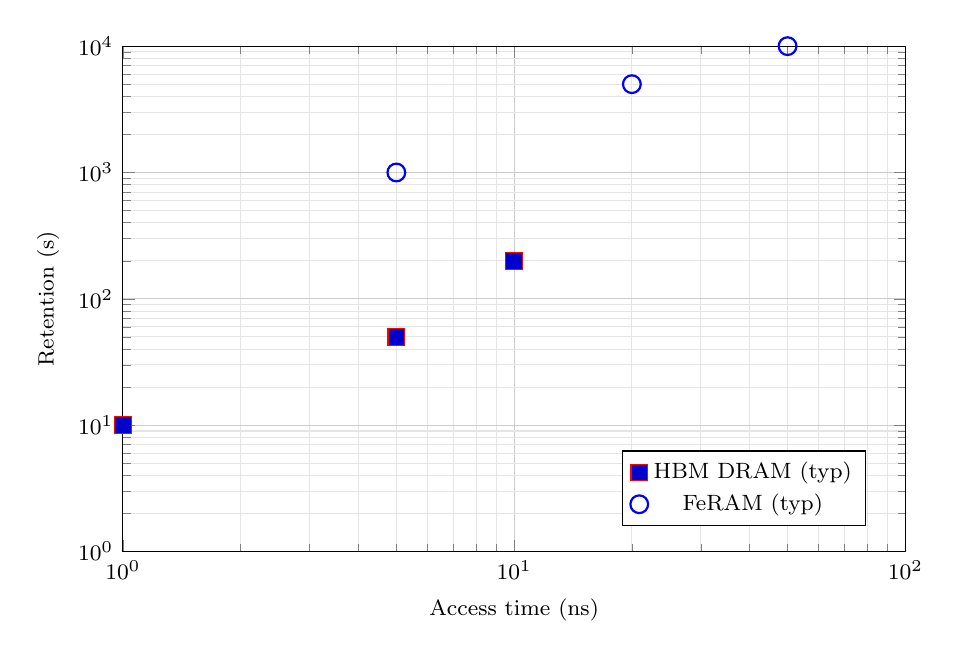
\begin{tikzpicture}
\begin{axis}[
    width=0.95\linewidth,   % 横幅をページ幅の95%に拡大
    height=8cm,             % 高さも拡大
    xlabel={Access time (ns)},
    ylabel={Retention (s)},
    xmode=log, ymode=log,
    xmin=1e0, xmax=1e2,
    ymin=1e0, ymax=1e4,
    grid=both,
    major grid style={gray!40},
    minor grid style={gray!20},
    legend style={
        at={(0.95,0.05)},     % グラフの右下
        anchor=south east,
        font=\footnotesize,
        fill=white,
        draw=black
    },
    tick label style={font=\footnotesize},
    label style={font=\footnotesize}
]

% HBM: 赤四角
\addplot+[only marks, mark=square*, mark size=3pt, red]
coordinates {(1, 10) (5, 50) (10, 200)};

% FeRAM: 青丸
\addplot+[only marks, mark=o, mark size=3.2pt, blue, thick]
coordinates {(5, 1e3) (20, 5e3) (50, 1e4)};

\legend{HBM DRAM (typ), FeRAM (typ)}
\end{axis}
\end{tikzpicture}
\caption{Access time vs. retention. Red squares: HBM; blue circles: FeRAM. Wider and taller view for clarity ($10^0$--$10^2$ ns, $10^0$--$10^4$ s).}
\label{fig:retention}
\end{figure}

\section{Discussion}
Table~\ref{tab:humanoid_comparison} compares the proposed Samizo-AITL PoC
with two representative humanoid platforms: Boston Dynamics \textit{Atlas} 
and Tesla \textit{Optimus}.
Atlas excels at dynamic acrobatics, while Optimus emphasizes scalable
industrial deployment. In contrast, the proposed PoC targets autonomy,
fault tolerance, and sustainable operation.

A first distinctive feature is the integration of LLMs into the hierarchical
control loop. Instead of replacing classical controllers, the LLM layer
generates goals, interprets anomalies, and provides conversational interfaces.
This complements the FSM for supervisory logic and PID/state-space methods
for stabilization, creating a hybrid architecture that combines the safety
of model-based control with the adaptability of data-driven intelligence.

A second differentiator is energy autonomy. The PoC integrates
piezoelectric, photovoltaic, and regenerative harvesting,
allowing up to 20\% of the power budget to be sustained
without external charging. This contrasts with Atlas and Optimus,
which rely exclusively on batteries. Together with FRAM/EEPROM-based
checkpoint-and-resume, the system ensures resilient operation
in remote or resource-limited environments.

A third contribution is educational reproducibility.
All specifications, models, and proof-of-concept results are openly published
in bilingual (Japanese–English) format on GitHub Pages.
This open-science approach enables replication, lowers barriers for students,
and positions the PoC as both a research prototype and an instructional
benchmark in control engineering education.

Overall, the proposed system demonstrates that hybrid architectures
can extend humanoid robotics beyond performance and manufacturability,
toward autonomy, resilience, and sustainable deployment.

\section{Conclusion}
This paper has proposed a Bio-Inkjet (Bio-IJ) architecture based on
bulk KNN actuators as a lead-free alternative to conventional PZT-based
printheads.
By combining multilayer KNN stacks, COF driver ICs, and silicon cavity
integration, the system achieves picoliter-scale droplet generation
under moderate voltages while ensuring material biocompatibility.

Unlike industrial printing, where full PZT compatibility in terms of
maximum $d_{33}$, billion-cycle endurance, and cost efficiency is
required, biomedical printing places emphasis on safety, controlled
droplet volume, and operational reliability over shorter lifetimes.
The proposed approach aligns well with these requirements, providing
sufficient performance for applications such as cell patterning,
protein microarrays, and hydrogel 3D fabrication.

These findings highlight bulk KNN as a practical foundation for
standardizing lead-free Bio-IJ systems in research, clinical, and
educational domains.
Future work will involve experimental validation of droplet formation,
long-term reliability testing under bio-relevant conditions, and system
integration with existing bioprinting workflows.

\textbf{Most importantly, this work emphasizes that in biomedical inkjet
printing, safety and biocompatibility must take precedence over extreme
performance metrics, positioning KNN-based Bio-IJ as a safe and viable
path toward Pb-free bioprinting.}


% ---- 文献
% どれも cite していないと .bbl が空になりコンパイルエラーになるので、
% 暫定で全件出力(ダミー)。実際に本文に \cite{...} を書けば \nocite は消してOK。
\nocite{*}
\bibliographystyle{IEEEtran}
\bibliography{refs}

% ---- Author Biography ----
\section*{Author Biography}
\noindent\textbf{Shinichi Samizo}
received the M.S. degree in Electrical and Electronic Engineering from Shinshu University, Japan.
He worked at Seiko Epson Corporation as an engineer in semiconductor memory and mixed-signal device development, and also contributed to inkjet MEMS actuators and PrecisionCore printhead technology.
He is currently an independent semiconductor researcher focusing on process/device education, memory architecture, and AI system integration.\\[2pt]
\textbf{Contact:} \href{mailto:shin3t72@gmail.com}{shin3t72@gmail.com}, \href{https://github.com/Samizo-AITL}{Samizo-AITL}

\end{document}
